% LatexEx1.tex - Project 1 MAS6001

\documentclass[a4paper, landscape, 20pt]{extreport}
\usepackage{amsmath}
\usepackage{extsizes}
\usepackage{amssymb}
\usepackage{natbib}
\usepackage{graphicx}
\usepackage{epstopdf}
\usepackage{geometry}
\usepackage{dcolumn}
\usepackage{appendix}
\usepackage{fixltx2e}
\usepackage{subfig}
\usepackage{float}
\usepackage{graphicx,wrapfig,lipsum}
\usepackage[usenames, dvipsnames]{color}
\usepackage{titlepic}

    \bibpunct[, ]{(}{)}{;}{a}{,}{,}

\title{\color{Blue} Non-Linear Relationships in Big Data}
\author{Julian Roche: 120103304 \\ \\ Supervisor: Dr Eleanor Stillman; Client: AstraZeneca }
\date{September 2015}

\graphicspath {{../../graphs/}}
\titlepic{\includegraphics[width=5.5cm,keepaspectratio]{tuoslogo_key_cmyk_med.jpg}}
\begin{document}
\pagestyle{myheadings}

\maketitle

\section*{\color{Blue} Introduction}

This project compared three different measures of association at identifying inter-variable relationships in large biological datasets. The three measures of association studied were:

\begin{itemize}
\item $A$ score, a probabilistic measure of association that generalises $R^2$.
\item Distance correlation ($dcor$), a measure of association based on pairwise distance between random variables.
\item Maximal Information Coefficient ($MIC$), an information theoretic measure of association.
\end{itemize}

The comparisons are based on power simulations and gene expression data comparing controls with Systematic Lupus Erythematosus (lupus) patients.

\newpage
\subsection*{\color{Blue} Simulation}
The simulations estimated the power of each association measure to detect statistical dependence for fifteen different functional forms while varying sample size, source distribution and the amount of additive noise.
	
\begin{figure}[H]
    \centering
    \subfloat{{\includegraphics[width=7cm]{FunctionFormsNoNoise.pdf} }}
    \qquad
    \subfloat{{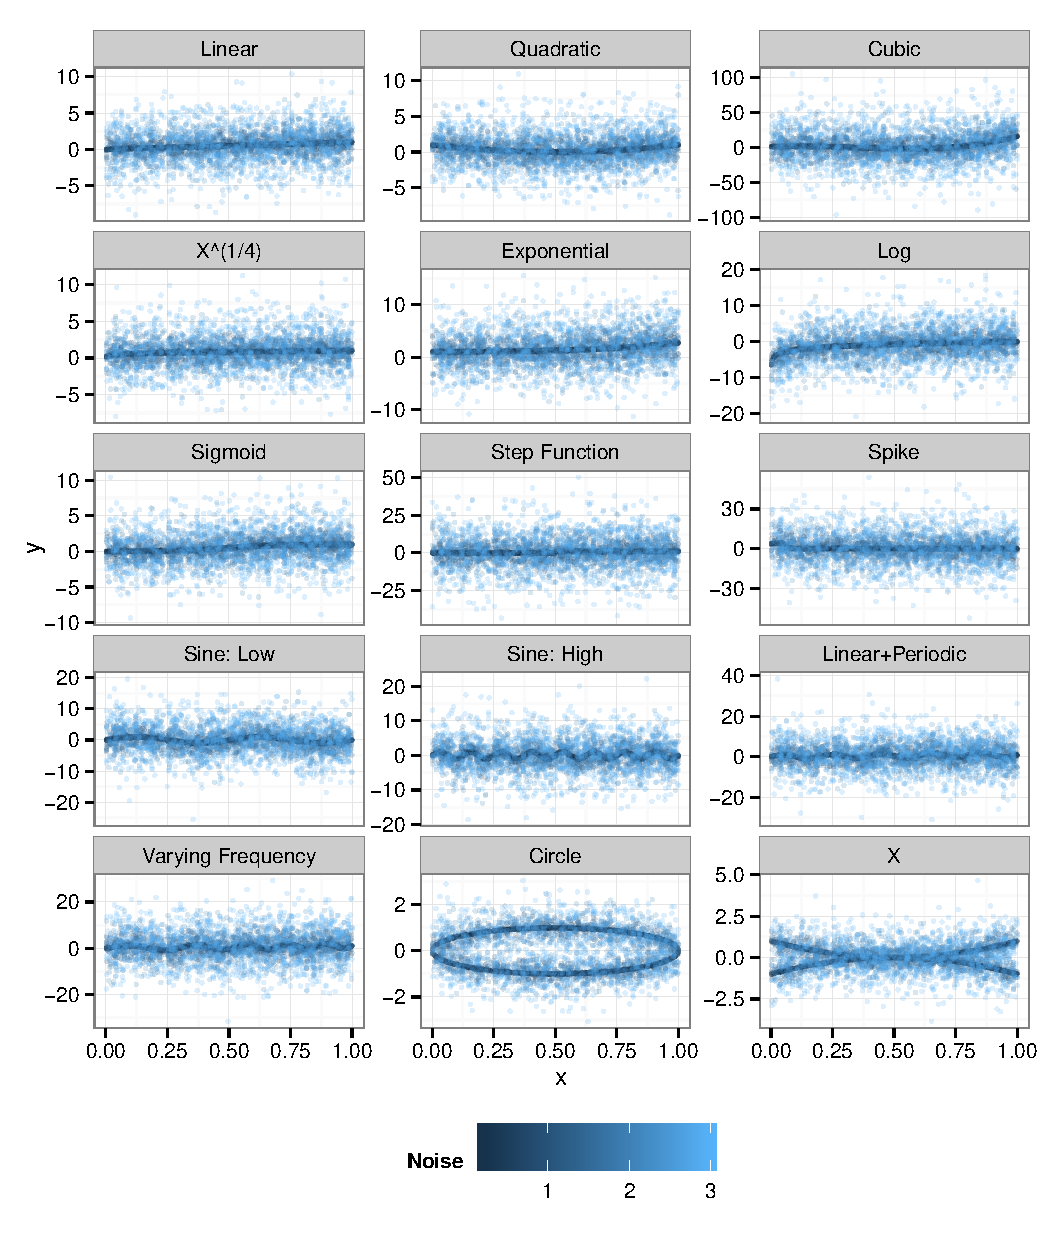
\includegraphics[width=7cm]{forms.pdf} }}
    \caption{The fifteen functional forms used before and after increasing noise has been added.}
\end{figure}

\subsection*{\color{Blue} Simulation}

\begin{figure}[H]
    \centering
    \subfloat[Power versus noise]{{\includegraphics[width=7cm,height=8cm]{power.pdf} }}%
    \qquad
    \subfloat[Power versus sample size]{{\includegraphics[width=7cm,height=8cm]{powerSizeUN10.pdf} }}%
\end{figure}

No measure exceeded all of the others in all of the cases but the simulation suggests that $dcor$ should perform better than either $MIC$ or $A$ on the basis of capacity to handle noise and deal with small samples. 

\newpage
\subsection*{\color{Blue} Gene Expression Analysis}

\begin{itemize}
\item The data is from an Affymetrix biochip. Each variable is a DNA probe which maps to one or more genes. 94 probes of biological interest were identified by the client. These were each given a numeric ID to simplify identification. Each sample is either a control or a lupus patient.

\item All two-way associations were analysed using $R^2$, $A$, $MIC$ and $dcor$.

\item The amount of non-linearity was estimated for each association measure, $\theta$, using:
	\begin{enumerate}
	\item Residual association ($r \theta$), the association of random variables after the linear relationship has been regressed out using a standard linear model. 
	\item Non-linear part of the association, $\theta - R^2$.
	\end{enumerate}
\end{itemize}

\subsection*{\color{Blue} Gene Expression Analysis}

\begin{itemize}
\item All three-way associations were analysed using $R^2$, $A$ and $dcor$ separately for lupus patients and controls and the amount of non-linearity was estimated as in the two-way case.

\item \textit{Multiple Adaptive Regression Splines} (MARS) were used to (a) provide an additional method of variable selection that could be contrasted to the association analysis, and (b) provide an additional method for investigating the amount of non-linearity present. MARS were chosen as they offer considerable flexibity in terms of variable interactions and how explanatory variables are treated, e.g. linearly or as `hinge' functions.

\item In order to assess the individual effect of genes (independently of associations), they were tested for differential expression between lupus patients and controls using the R package $limma$. FDR adjusted $p$-values were used to mitigate the false discovery rate.
\end{itemize}

\subsection*{\color{Blue} Gene Expression Data}
\begin{figure}[H]
	\begin{center}
		\includegraphics[width=12cm]{heat3}
\caption{Heatmap of the data using $1 - dcor$ for clustering. Columns represent probes and rows samples. The band on the top represents chromosomes. The band on the left represents controls (green) and lupus patients (orange).}
	\end{center}
\end{figure}

\newpage

\newpage
\subsection*{\color{Blue} Differences in Association Measures}

\begin{figure}[H]
    \centering
    \subfloat[Two-way]{{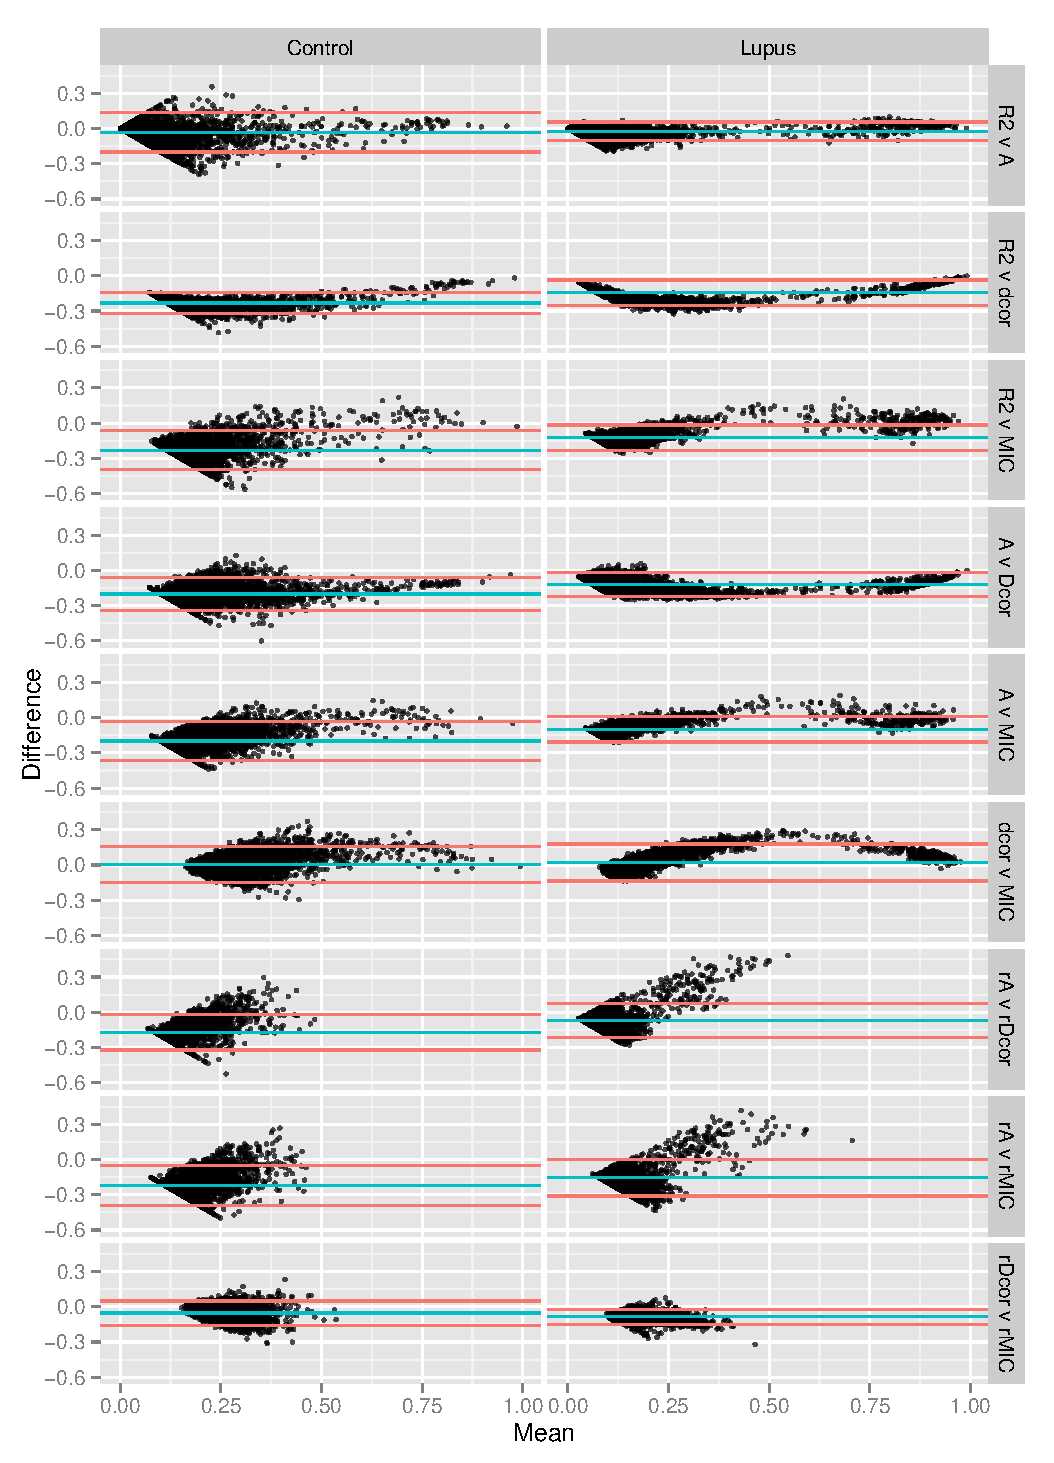
\includegraphics[width=6cm]{mdAssociations2} }}%
    \qquad
    \subfloat[Three-way]{{\includegraphics[width=6cm]{3ba2} }}%
    \caption{Bland-Altman plots comparing each measure of association.}
\end{figure}


$dcor$ appears to be biased upwards from $R^2$ but has a high concordance with $R^2$ as measured by Kendall's $\tau$. 
\newpage
\subsection*{\color{Blue} Differences between Lupus and Controls}

\begin{figure}[H]
	\begin{center}
		\includegraphics[width=12cm]{2wayTop}
\caption{Eighteen two-way associations identified in lupus patients ordered by non-linear part of association. Lupus patients are in blue while controls are in red. The axes labels are the probe IDs.}
	\end{center}
\end{figure}

\subsection*{\color{Blue} Three-way Results}

\begin{itemize}
\item The three-way analysis produced many strong associations however most of these were an artefact arising from the fact that if two variables are strongly associated the extra information provided by a third variable necessarily increases the association. 

\item A simple strategy to deal with this is to filter by criteria such as whether or not all genes are differentially expressed.
\item Twelve strong three-way associations were identified involving differentially expressed genes.

\end{itemize}

\subsection*{\color{Blue} Three-way Results}

\begin{figure}[H]
	\begin{center}
		\includegraphics[width=12cm]{3wayFilter}
\caption{Four different filter strategies for three-way associations. Each plot shows the frequency of probe involvement in three-way associations.}
	\end{center}
\end{figure}

\newpage
\section*{\color{Blue} Conclusions}

\begin{itemize}
\item Simulation showed that no one measure of association had greater power to measure association in all cases but that a combination of $A$ and $dcor$ should be able to identify non-linear associations.


\item $dcor$ identified all strong associations identified by $A$ in the two-way case. $R^2 \cup dcor$  identified all strong associations identified by $A$ in the three-way case. 

\item No significant non-linearities were identified. The non-linear part of association in relationships of interest was between 10\% and 15\%.

\item There is strong evidence that twenty two genes are differentially expressed between lupus patients and controls. Fifteen of these were involved in eighteen strong ($\ge 0.90$) two-way associations. These were located on eleven different chromosomes.
\end{itemize}

\end{document}

